%% LyX 2.2.2 created this file.  For more info, see http://www.lyx.org/.
%% Do not edit unless you really know what you are doing.
\documentclass[english]{beamer}
\usepackage{mathptmx}
\usepackage[latin9]{inputenc}
\usepackage{amsmath}
\usepackage{amssymb}
\usepackage{graphicx}
\usepackage[european]{circuitikz}
\usepackage{bookmark}
\ctikzset{tripoles/mos style/arrows}

\makeatletter

%%%%%%%%%%%%%%%%%%%%%%%%%%%%%% LyX specific LaTeX commands.
%% Because html converters don't know tabularnewline
\providecommand{\tabularnewline}{\\}

%%%%%%%%%%%%%%%%%%%%%%%%%%%%%% Textclass specific LaTeX commands.
 % this default might be overridden by plain title style
 \newcommand\makebeamertitle{\frame{\maketitle}}%
 % (ERT) argument for the TOC
 \AtBeginDocument{%
   \let\origtableofcontents=\tableofcontents
   \def\tableofcontents{\@ifnextchar[{\origtableofcontents}{\gobbletableofcontents}}
   \def\gobbletableofcontents#1{\origtableofcontents}
 }

%%%%%%%%%%%%%%%%%%%%%%%%%%%%%% User specified LaTeX commands.
\usetheme{Warsaw}
% or ...

\setbeamercovered{transparent}
% or whatever (possibly just delete it)

\makeatother

\usepackage{babel}
\begin{document}

\title[Designing a SCaM]{Analog Design for a Single-Chip atto Mote (SCaM) Microcontroller
}

\author[Kevavi]{Kevin Chen, Avi Pandey, Kevin Zheng}

\institute{University of California, Berkeley}

\date{Final Presentation}

\makebeamertitle

%\pgfdeclareimage[height=0.5cm]{institution-logo}{logo.png}
%\logo{\pgfuseimage{institution-logo}}

\AtBeginSubsection[]{%
  \frame<beamer>{ 
    \frametitle{Outline}   
    \tableofcontents[currentsection,currentsubsection] 
  }
}

%\beamerdefaultoverlayspecification{<+->}
\begin{frame}{Outline}

\tableofcontents{}
\end{frame}

\section{Overview}

\subsection{Introduction}

\begin{frame}{Block Diagram}
\begin{figure}
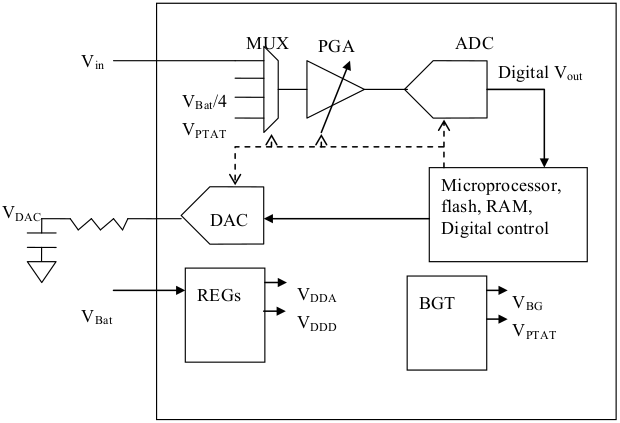
\includegraphics[width=0.7\linewidth]{block-diagram}
\end{figure}
\end{frame}

\subsection{Results}

\begin{frame}{Summary of Results}
\begin{block}{Scoring}
\begin{itemize}
    \item 5\%: Meeting internal milestone dates
    \item 40\%: Functional SCaM system
    \item 55\%: Functional SCaM units meeting specs
\end{itemize}
\end{block}
%
\begin{block}{Our Results}
\begin{itemize}
    \item All milestones met on-time
    \item SCaM is alive
    \item SCaM behaves moderately well under most conditions
\end{itemize}
\end{block}
\end{frame}

\begin{frame}{Key Performance Metrics}
\begin{itemize}
    \item Worst-case error: 3 LSB
    \item Average power consumption: 11 mW
    \item Die size: 0.1639 mm$^2$
    \item Unit cost: 1.64 cents (without packaging)
    \item Minimum supply for $<3$ LSB error: 1.4 V
\end{itemize}
\end{frame}

\begin{frame}{Overall System Error (Low Inputs)}
400 mV x1 / 100 mV x4 / 50 mV x8
\begin{tabular}{|c|c|c|c|}
    \hline
    Temp (C) & 1.6 V    & 2.4 V         & 3.2 V      \tabularnewline \hline
    0  & 1 / 2 / 2      & 1 / 1 / 2     & 0 / 1 / 2 \tabularnewline
    \hline
    25 & 1 / 1 /   2    & 1 / 1 / 2     & 0 / 1 / 2 \tabularnewline
    \hline
    70 & 0 / 1 / 2      & 0 / 1 / 2     & 0 / 1 / 2 \tabularnewline
    \hline
\end{tabular}
\end{frame}
%

\begin{frame}{Overall System Error (High Inputs)}
800 mV x1 / 200 mV x4 / 100 mV x8
\begin{tabular}{|c|c|c|c|}
    \hline
    Temp (C) & 1.6 V    & 2.4 V         & 3.2 V      \tabularnewline \hline
    0  &   2 / 2 / 2    & 2 / 1 / 1     & 2 / 1 / 1  \tabularnewline
    \hline
    25 &   2 / 1 / 2    & 2 / 1 / 2     & 2 / 1 / 1  \tabularnewline
    \hline
    70 &   2 / 1 / 2    & 2 / 1 / 2     & 3 / 1 / 2  \tabularnewline
    \hline
\end{tabular}
\end{frame}
%

\begin{frame}{Areas and Costs}
\begin{center}
\begin{tabular}{|c|c|}
\hline
Block & Size (mm$^2$) \tabularnewline \hline
BGT & 0.0575\tabularnewline \hline
REG/REF & 0.00044\tabularnewline \hline
MUX & 3.6*$10^{-6}$\tabularnewline \hline
PGA & 0.0665 \tabularnewline \hline
ADC* & 0.0021 \tabularnewline \hline
Total & 0.1639 \tabularnewline \hline
\end{tabular}
\begin{itemize}
\item ADC area does not include SAR state machine area
\item Area is dominated by capacitive array in the PGA, and the resistors used in the band gap circuit
\item Die cost comes out to 1.64 cents
\end{itemize}
\end{center}
\end{frame}

\begin{frame}{Error Summary (Excuses)}
During our final stages of design, we ran into some major issues that either arose from complete integration of fully implemented components, or were recurring problems that impacted performance, including:
\begin{itemize}
\item Band gap reference was unreliable
\item Temperature sensor gave outputs that were too high for PGA's CM input
\item Too much variation on V$_{dd,a}$ and V$_{ref}$
\item Output of PGA was drooping, due to leakage of charge
\end{itemize}
\end{frame}

%

\section{Blocks}

\subsection{Band Gap}

\begin{frame}{Band Gap}
\begin{block}{Constraints and Target Specs}
\begin{itemize}
    \item Temperature/supply-independent ~1.2 V output
    \item Accurate 1.000 V reference voltage output
    \item Supports PTAT current generation
    \item High supply noise rejection
\end{itemize}
\end{block}
\begin{block}{Design Choices}
\begin{itemize}
    \item Modified enhanced power supply rejection bandgap reference from
        Yao, Guo 2009
    \item Internally-compensated two-stage PMOS-input error amplifier with
        constant gm bias
    \item Startup circuit in PSR reject branch to improve startup
\end{itemize}
\end{block}
\end{frame}
%
\begin{frame}{Design}
\begin{itemize}
    \item $V_{ref} = V_{th} \ln(n) \frac{R2}{R1} + V_{be}$
    \item $V_{be}$ has a coefficient of -1.8 mV/K for our diodes
    \item Sets $V_{be} = $ 662.4 mV
    \item For $n = 8$, $\frac{R2}{R1} = 10$, actual ratio $\approx 8.5$
    \item For max size diodes, $I = 600$ nA for our $V_{be}$
\end{itemize}
\end{frame}

\begin{frame}{Schematic}
\begin{center}
    \begin{circuitikz}[scale=0.5, transform shape, american resistors]
    \draw
    (0,5) node[pmos, xscale=-1](pmos1){}
    (pmos1.S) -- (0,6)
    (3,5) node[pmos](pmos2){}
    (pmos2.S) -- (3,6)
    (pmos1.G) -- (pmos2.G)
    (pmos1.D) -- (0,4)
    (pmos2.D) -- (3,4)
   
    (0,4) to [R] ++(0,-2)
    to [R] ++(0,-2)
    to [Do] ++(0,-2)

    (3,4) to [R] ++(0,-2)
    to [short] ++(0,-2)
    to [Do] ++(0,-2)
    to[short] ++(-5,0)
    
    (-2,-2) to[R] ++(0,3)
    to[R] ++(0,3)
    -| (pmos1.D)

    (6,-2) to[R] ++(0,3)
    to[R] ++(0,3)
    -| (pmos2.D)

    (6,4) to[short,-o] ++(0.5, 0)
    node[anchor=west]{$V_{bg}$}
    (4,4) to[C] ++(0,-6)
    
    (6,1) to[short,-o] ++(0.5, 0)
    node[anchor=west]{$V_{ref}$}
    
    (0,2) to[short,-o] ++(0.3,0)
    node[anchor=west]{-}
    (3,2) to[short,-o] ++(-0.3,0)
    node[anchor=east]{+}

    (0,-2) to[short] ++(6,0)   
    (0,6) to[short] ++(3,0)

    (10,0) node[op amp](opamp1){}
    (12,0) node[nmos](nmos1){}
    (opamp1.out) |- (nmos1.G)
    (nmos1.S)  |- (0,-2)
    (12,5) node[pmos](pmos3){}
    (pmos3.D) -- (nmos1.D)
    (pmos3.D) -| (pmos3.G)
    (pmos3.S) |- (0,6)
    
    (pmos3.G) node[anchor=east] {$V_b$}
    (pmos1.G) to[short] ++(0.5,0)
    node[anchor=north]{$V_b$}

    (14,5) node[pmos](pmos4){}
    (pmos4.G) node[anchor=east] {$V_b$}
    (pmos4.D) to[R] (14,-2)
    (pmos4.S) |- (0,6)
    (0,-2) to[short] (14,-2)
    (14,2) to[short, -o] ++(0.5,0)
    node[anchor=west] {$V_{temp}$}
    ;
\end{circuitikz}
    

\end{center}
\end{frame}
%
\begin{frame}{Schematic}
\begin{center}
    
\begin{circuitikz}[scale=0.5, transform shape, american resistors]
    \draw
    (0,5) node[pmos, xscale=-1](pmos1){}
    (pmos1.S) -- (0,6)
    (3,5) node[pmos](pmos2){}
    (pmos2.S) -- (3,6)
    (pmos1.G) -- (pmos2.G)
    (pmos1.D) -- (0,4)
    (pmos2.D) -- (3,4)
   
    (0,4) to [R] ++(0,-2)
    to [R] ++(0,-2)
    to [Do] ++(0,-2)

    (3,4) to [R] ++(0,-2)
    to [short] ++(0,-2)
    to [Do] ++(0,-2)
    to[short] ++(-5,0)
    
    (-2,-2) to[R] ++(0,3)
    to[R] ++(0,3)
    -| (pmos1.D)

    (6,-2) to[R] ++(0,3)
    to[R] ++(0,3)
    -| (pmos2.D)

    (6,4) to[short,-o] ++(0.5, 0)
    node[anchor=west]{$V_{bg}$}
    (4,4) to[C] ++(0,-6)
    
    (6,1) to[short,-o] ++(0.5, 0)
    node[anchor=west]{$V_{ref}$}
    
    (0,2) to[short,-o] ++(0.3,0)
    node[anchor=west]{-}
    (3,2) to[short,-o] ++(-0.3,0)
    node[anchor=east]{+}

    (0,-2) to[short] ++(6,0)   
    (0,6) to[short] ++(3,0)

    (10,0) node[op amp](opamp1){}
    (12,0) node[nmos](nmos1){}
    (opamp1.out) |- (nmos1.G)
    (nmos1.S)  |- (0,-2)
    (12,5) node[pmos](pmos3){}
    (pmos3.D) -- (nmos1.D)
    (pmos3.D) -| (pmos3.G)
    (pmos3.S) |- (0,6)
    
    (pmos3.G) node[anchor=east] {$V_b$}
    (pmos1.G) to[short] ++(0.5,0)
    node[anchor=north]{$V_b$}
    
    (13,0) node[nmos, xscale=-1](nmos2){}
    (nmos2.S) |- (12,-2)
    (nmos2.D) |- (12,2.5)

    (16,0) node[nmos](nmos3){}
    (16,5) node[pmos, xscale=-1](pmos5){}
    (nmos3.S) |- (12,-2)
    (nmos3.D) -- (pmos5.D)
    (nmos3.G) to[short,-o] ++(-0.2,0)
    node[anchor=east]{$V_b$}
    (nmos2.G) |- (nmos3.D)
    (pmos5.S) |- (0,6)

    (19,5) node[pmos](pmos6){}
    (pmos6.S) |- (0,6)
    (pmos6.G) -- (pmos5.G) 
    (pmos6.D) to[C] (19,-2)

    (18,3) node[pmos](pmos7){}
    (pmos7.G) |- (18,6)
    (pmos7.S) |- (pmos6.G)
    (pmos7.S) -| (pmos6.D)
    (pmos7.D) -- (18,-2)
    ;
\end{circuitikz}
    

\end{center}
\end{frame}
%
\begin{frame}{Performance}
\begin{itemize}
    \item Reference voltage variation of 3.6 mV between 0-70 C
    \item Temperature sensor is broken (always above 1 V)
\end{itemize}
\begin{figure}
    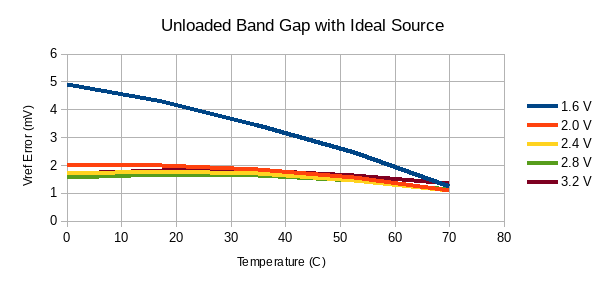
\includegraphics[width=\linewidth]{bg_data/vt-variation-final.png}
\end{figure}
\end{frame}

\begin{frame}{Lessons Learned}
\begin{itemize}
    \item Something happened between revisions 1.2.3 and 1.3.0
    \item Nobody caught the change...
    \item We should have stuck with 1.2.3, working temp sensor
\end{itemize}
\begin{figure}
    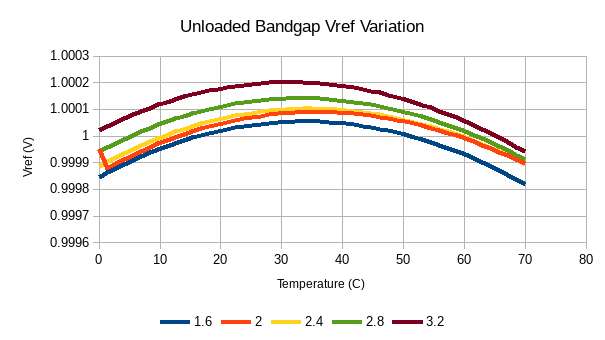
\includegraphics[width=\linewidth]{bg_data/vt-variation.png}
\end{figure}
\end{frame}
%

\subsection{Regulators}

\begin{frame}{Voltage Regulator Topology}
\begin{itemize}
\item Used general LDO topology, with a large pass transistor
\end{itemize}
\end{frame}

\begin{frame}{Digital Regulator Design}
\begin{block}{Op-amp Considerations}
\begin{itemize}
\item{NMOS one stage op amp}
\begin{itemize}
\item{No substantial compensation required}
\end{itemize}
\item{Used smaller L values, specifically 600nm, to speed up amplifier response}
\
\end{itemize}
\end{block}
\end{frame}

\begin{frame}{Analog Regulator Design}
\begin{block}{Op-amp Considerations}
\begin{itemize}
\item Used exact same op-amp as DREG, as it happened to be fast enough to satisfy the AREG load
\item Changed the pass transistor to be slightly smaller
\end{itemize}
\end{block}
\end{frame}
%

\begin{frame}{Voltage Reference}
\begin{itemize}
\item Used a unity gain buffer after a resistively divided $V_{bg}$
\begin{itemize}
\item Op-amp used NMOS two stage topology to satisfy minimal gain error, and had 100fF compensation to maintain stability
\item Second stage used larger $\frac{W}{L}$ to supply more current to keep the op-amp going fast, and combat spikes in current draw during ADC loads
\end{itemize}
\end{itemize}
\end{frame}

\subsection{PGA}

\begin{frame}{PGA Topology}
\begin{block}{Switched Cap Array Topology}
\begin{itemize}
\item Base cap size of 8pF, prevents leakage from affecting voltage
\item Extra switch required for convergence (more on this later)  
\end{itemize}
\end{block}
\begin{center}
    \begin{circuitikz} [scale=0.5, transform shape]
    \draw
    (0,0)
    node[op amp](opamp1){}
    (opamp1.out) -| (1.5,2)
    to [C] ++(-3,0)
    (-1.5,2) |- (opamp1.-)
    (-1.5,2) to[short] ++(0,2)
    to [spst, l_=$\phi_1$] ++(3,0)
    to [short] ++(0,-2)
    
    (opamp1.-) -- (-3,0.5)
    (-3,0.5) to[C] ++(-2,0)
    to[short] ++(-2,0)
    (-3,0.5) to[short] ++(0,2)
    to[C] ++(-2,0)
    to[spst, l_=$\phi_1 B_0$] ++(-2,0)
    (-3,0.5) to[short] ++(0,4)
    to[C] ++(-2,0)
    to[spst, l_=$\phi_1 B_1$] ++(-2,0)
    (-3,0.5) to[short] ++(0,6)
    to[C] ++(-2,0)
    to[spst, l_=$\phi_1 B_2$] ++(-2,0)
    to[short] ++(0,-6)
    to[spst, l_=$\phi_2$] ++(0,-2)
    node[ground]{}

    (-7,0.5) to[spst, -o, l_=$\phi_1$] ++(-2,0)
    node[anchor=east]{$V_{in}$}
    
    (-3,0.5) to[spst, l_=$\phi_1$] ++(0,-2)
    node[ground]{}
    
    (opamp1.+) -| (-1.5,-1.5) node[ground]{}
    ;
\end{circuitikz}

\end{center}
\end{frame}
%
\begin{frame}{PGA Design}
\begin{block}{Op-amp topology}
\begin{itemize}
\item Used a PMOS input folded cascode with PMOS second stage
\item Large capacitors in PGA require large output stage
\end{itemize}
\end{block}
\begin{center}
     \begin{circuitikz}[scale = 0.5, transform shape]
        \draw
        (2,5) node[pmos](m6) {} 
        node [anchor=west]{$\frac{4\mu m}{1\mu m}$}
        (1,3) node[pmos](m1a) {}
        node [anchor=west]{$\frac{2\mu m}{1\mu m}$}
        (3,3) node[pmos, xscale=-1](m1b) {}
        (m6.D) -| (m1a.S)
        (m6.D) -| (m1b.S)

        (m1a.D) to[short] ++(0,-2)
        (m1b.D) to[short] ++(0,-2)

        (5,5) node[pmos, xscale=-1](m4a) {}
        (8,5) node[pmos](m4b) {}
        node [anchor=west]{$\frac{2\mu m}{1\mu m}$}
        (5,3) node[pmos, xscale=-1](m3a) {}
        (8,3) node[pmos](m3b) {}
        node [anchor=west]{$\frac{2\mu m}{1\mu m}$}
        
        (m4a.G) -- (m4b.G)
        (m3a.G) -- (m3b.G)
        (m4a.D) -- (m3a.S)
        (m4b.D) -- (m3b.S)
        (m4a.G) |- (m3a.D)
        (m3a.G) to[short] ++(0.5,0)
        node[anchor=north]{$V_{B4}$}
        
        (5,1) node[nmos, xscale=-1](m2a){}
        (8,1) node[nmos](m2b){}
        node [anchor=west]{$\frac{1\mu m}{1\mu m}$}
        (5,-1) node[nmos, xscale=-1](m5a){}
        (8,-1) node[nmos](m5b){}
        node [anchor=west]{$\frac{2\mu m}{1\mu m}$}

        (m5a.G) -- (m5b.G)
        (m2a.G) -- (m2b.G)
        (m2a.S) -- (m5a.D)
        (m2b.S) -- (m5b.D)

        (m2a.D) -- (m3a.D)
        (m2b.D) -- (m3b.D)
        (m1b.D) to[short] ++(0,-2)
        -| (m5b.D)
        (m1a.D) to[short] ++(0,-2.5) 
        -| (m5a.D)
        (m6.S) -- (m4a.S)
        (m6.S) -- (m4b.S)
        (m6.S) to[short] ++(-0.5,0)
        (m4b.S) to[short] ++(0.5,0)
        
        (m5a.S) -- (m5b.S)
        (m5a.S) to[short] ++(-3.5,0)
        (m5b.S) to[short] ++(0.5,0)
        
        (m1a.G) node[anchor=east]{$V_-$}
        (m1b.G) node[anchor=west]{$V_+$}
        
        (m6.G) node[anchor=east]{$V_{B1}$}
        (m5a.G) to[short] ++(0.5,0)
        node[anchor=south]{$V_{B2}$}
        (m2a.G) to[short] ++(0.5,0)
        node[anchor=south]{$V_{B3}$}
        (m4a.S) node[anchor=south]{$V_\text{DD}$}
        (m5a.S) node[anchor=north]{GND}

        (11,-1) node[nmos](nmosa){}
        node[anchor=west]{$\frac{1\mu m}{1\mu m}$} 
        (11,5) node[pmos](pmosa){}
        node[anchor=west]{$\frac{1\mu m}{1\mu m}$}
        (nmosa.D) -- (pmosa.D)
        (nmosa.S) -- (m5a.S)
        (pmosa.S) -- (m4b.S)
        (nmosa.G) node[anchor=east]{$V_{B2}$}
        (pmosa.G) |- (8,2)
        ;
    \end{circuitikz}

\end{center}
\end{frame}
%
\begin{frame}{PGA Design}
\begin{block}{PGA Performance}
\begin{itemize}
    \item For low input voltages, the PGA performs as exptected
    \item Many mV of error for high inputs in Unity Gain
\end{itemize}
\end{block}
\begin{center}
    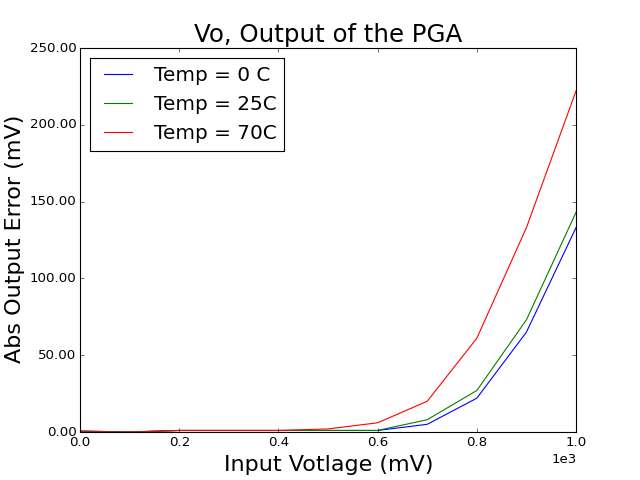
\includegraphics[scale=0.29]{PGA_v2_data/PGA_trans_out/figure.png}
\end{center}
\end{frame}
%
\begin{frame}{PGA Design}
\begin{block}{PGA Leakage}
\begin{itemize}
    \item Majority of Leakage occurs through switches at the $V^-$ node
    \item $V^-$ drops to -450mV in unity gain
\end{itemize}
\end{block}
\end{frame}
%
\begin{frame}{PGA Design}
\begin{block}{Charge Pump}
\begin{itemize}
    \item Adding a charge pump to the feedback switch prevents leakage
    \item Charge pump is same topology as in Scott et al. 
\end{itemize}
\end{block}
\begin{center}
    \begin{circuitikz}[scale=0.4, transform shape]
    \draw
    (0,0) node[nmos, rotate=90, yscale=-1](pmos1){}
    (pmos1.S) to[short] ++(-2,0)
    
    (-1,1.5) node[nmos, rotate=90, yscale=-1](nmos1){}
    (nmos1.G) -| (nmos1.D)
    (nmos1.D) to[short] ++(0.28,0)
    to[short] ++(0,-1.9)
    (nmos1.S) to[short] ++(-0.5,0)
    node[ground]{}  
    
    (1,-1.5) node[nmos, rotate=90, yscale=-1](pmos2){}
    (pmos2.S) -| (pmos1.G)
    (pmos2.D) to[short] (3,-1.5)
    |- (nmos1.S)    
    
    (0,-3.5) node[pmos, xscale=-1, yscale=-1](nmos2){}
    (nmos2.D) -- (pmos1.G)
    (nmos2.G) -| (pmos2.G)
    
    (1, -5) node[american not port, rotate=90](inv1) {}
    (inv1.out) |- (nmos2.G)
    (inv1.in) -| (nmos2.S)
    (inv1.in) -| (3,-3.5)
    (3,-3.5) to[C, l_=$C_{hold}$] ++(0,2)
    
    (inv1.in) to[short,-o] ++(0,-0.5)
    node[anchor=west]{phi\_1}

    (pmos1.D) to[short] ++(4,0)
    ;
\end{circuitikz}

\end{center}
\end{frame}
%
\subsection{ADC}

\begin{frame}{ADC Topology}
\begin{block}{Basic Performance}
\begin{itemize}
\item Uses a 10MHz digital clock
\end{itemize}
\end{block}
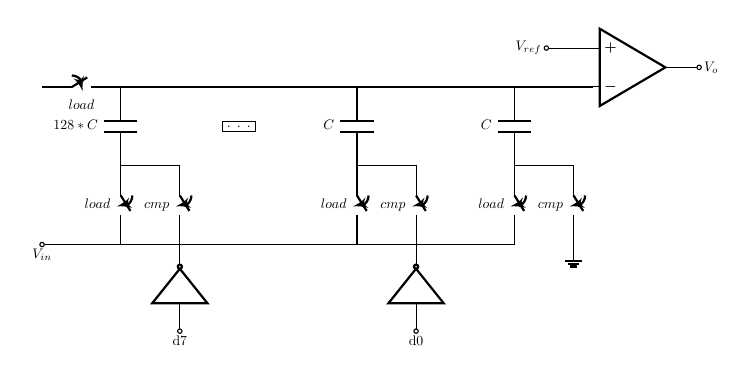
\begin{tikzpicture}[scale = 0.5, transform shape]
    \draw
    (0,4) 
    to[spst, l_=$load$] ++(2,0)
    to[short] ++(12,0)
    
    (2,4)
    to[C, l_=$128*C$] ++(0,-2)
    to[spst, l_=$load$] ++(0,-2)
    to[short, -o] ++(-2,0)
    node[anchor=north]{$V_{in}$}
    
    (2,2)
    to[short] ++(1.5,0)
    to[spst, l_=$cmp$] ++(0,-2)
    
    (3.5,-1)
    node[american not port, rotate = 90] (inv1) {}
    (inv1.out) -- (3.5,0)
    (inv1.in) to[short, -o] ++(0,-0.5)
    node[anchor=north]{d7}
    
    (8,4)
    to[C, l_=$C$] ++(0,-2)
    to[spst, l_=$load$] ++(0,-2)
    to[short] (0,0)
    
    (8,2)
    to[short] ++(1.5,0)
    to[spst, l_=$cmp$] ++(0,-2)
    
    (9.5,-1)
    node[american not port, rotate = 90] (inv1) {}
    (inv1.out) -- (9.5,0)
    (inv1.in) to[short, -o] ++(0,-0.5)
    node[anchor=north]{d0}

    
    (12,4)
    to[C, l_=$C$] ++(0,-2)
    to[spst, l_=$load$] ++(0,-2)
    to[short] (0,0)
    
    (12,2)
    to[short] ++(1.5,0)
    to[spst, l_=$cmp$] ++(0,-2)
    node[ground]{}

    (15,4.5) node[op amp, yscale=-1](comp){} 
    (comp.+) to[short, -o] ++(-1,0)
    node[anchor=east]{$V_{ref}$}
    
    (comp.out) to[short,-o] ++(0.5,0)
    node[anchor=west]{$V_o$}

    node[draw] at (5,3) {. . .}
    ;
\end{tikzpicture}

\end{frame}
%
\begin{frame}{ADC - Leakage}
\begin{block}{Charge Leakage}
\begin{itemize}
\item d7 and d6 overlap (thanks Brad), causes unexpectadly high voltages
\item High leakage current causes more than an LSB of loss.
\end{itemize}
\end{block}
\begin{figure}
\begin{minipage}{.5\textwidth}
    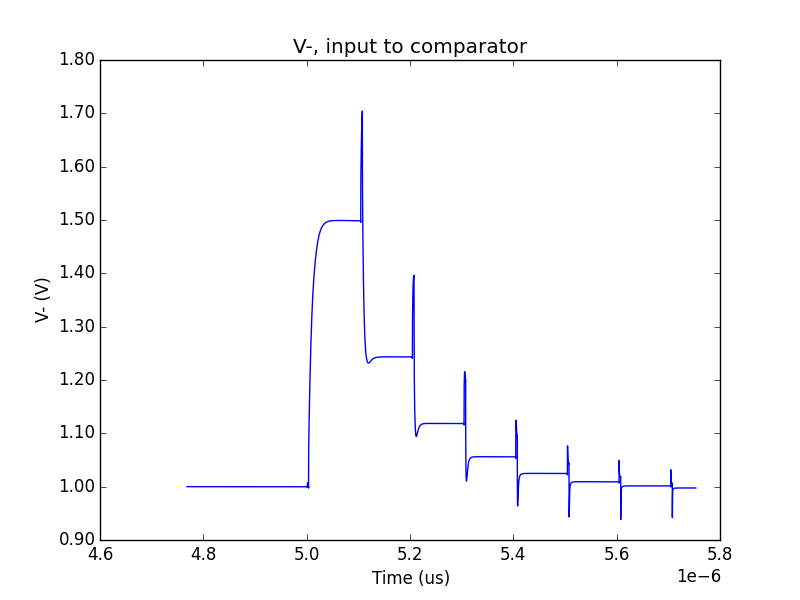
\includegraphics[scale=0.29]{ADC_data/Version2/figure_1.png} 
\end{minipage}%
\begin{minipage}{.5\textwidth}
    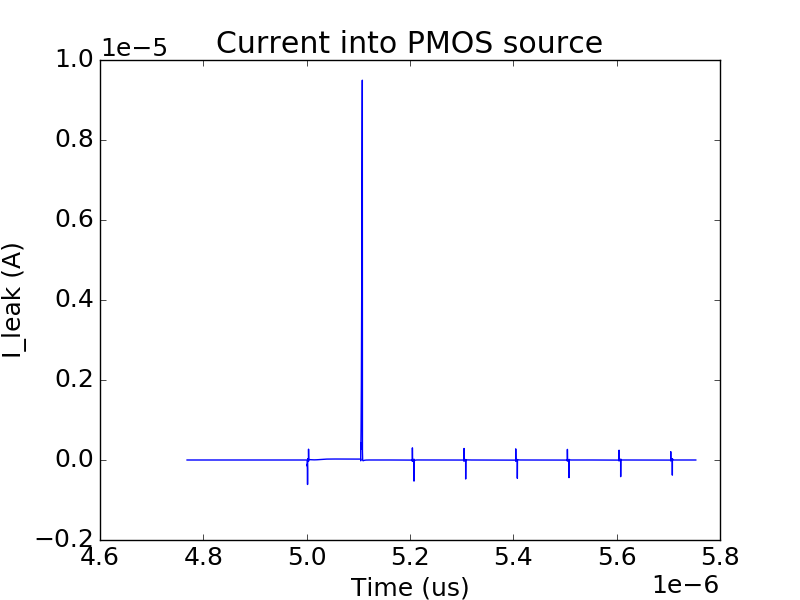
\includegraphics[scale=0.29]{ADC_data/Version2/figure_2.png}
\end{minipage}
\end{figure}
\end{frame}

\begin{frame}{ADC- Charge Pump}
\begin{block}{Charge Pump Topolgy}
\begin{itemize}
\item Using a charge pump to reduce the $V_{GS}$ of the Load PMOS
\item Restricts leakage to less than an LSB
\end{itemize}
\end{block}
\begin{center}
\begin{circuitikz}[scale=0.4, transform shape]
    \draw
    (0,0) node[pmos, rotate=90](pmos1){}
    (pmos1.S) to[short,-o] ++(-1,0)
    node[anchor=north]{$V_{ref}$}
    
    (-1,1.5) node[nmos,rotate=90](nmos1){}
    (pmos1.S) to[short] ++(-1,0)
    |- (nmos1.D)
    (nmos1.G) -| (-1.8,0.5)
    (nmos1.S) to[short] ++(0.28,0)
    to[short] ++(0,-1.9)  
    
    (1,-1.5) node[pmos, rotate=90](pmos2){}
    (pmos2.S) -| (pmos1.G)
    (pmos2.D) to[short] (3,-1.5)
    |- (nmos1.S)    
    
    (0,-3.5) node[nmos, xscale=-1](nmos2){}
    (nmos2.D) -- (pmos1.G)
    (nmos2.G) -| (pmos2.G)
    
    (1, -5) node[american not port, rotate=90](inv1) {}
    (inv1.out) |- (nmos2.G)
    (inv1.in) -| (nmos2.S)
    (inv1.in) -| (3,-3.5)
    (3,-3.5) to[C, l_=$C_{hold}$] ++(0,2)
    
    (inv1.in) to[short,-o] ++(0,-0.5)
    node[anchor=west]{load\_b}

    (pmos1.D) to[short] ++(4,0)
    ;
\end{circuitikz}

\end{center}
\end{frame}

\begin{frame}{ADC - Charge Pump cont.}
\begin{figure}
\begin{minipage}{.5\textwidth}
    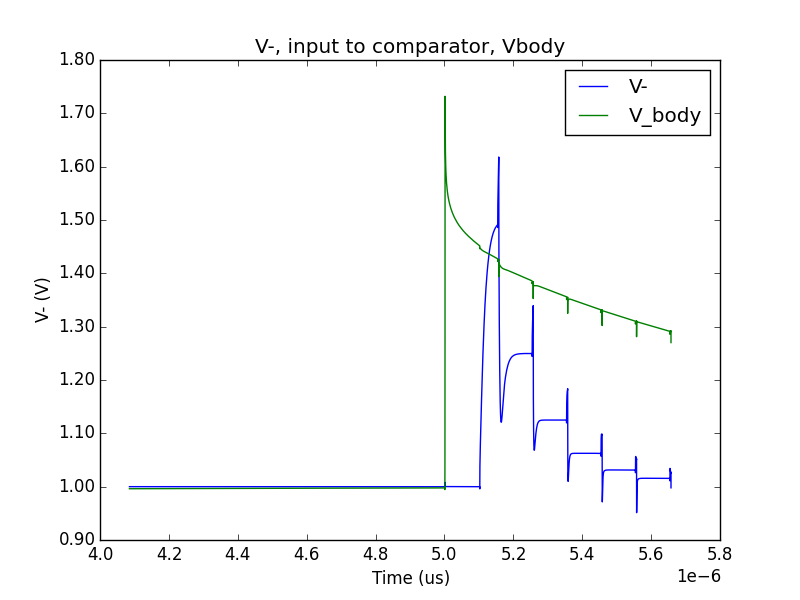
\includegraphics[scale=0.29]{ADC_data/Version3/figure_1.png} 
\end{minipage}%
\begin{minipage}{.5\textwidth}
    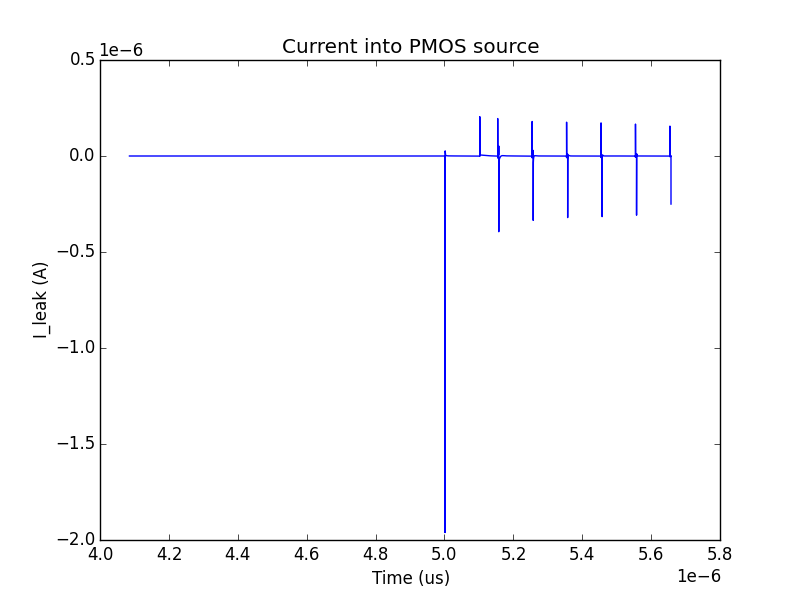
\includegraphics[scale=0.29]{ADC_data/Version3/figure_2.png}
\end{minipage}
\end{figure}
\end{frame}

\begin{frame}{Comparator}
\begin{block}{Constraints and Target Specs}
\begin{itemize}
    \item Fast enough
    \item Low input offset voltage
\end{itemize}
\end{block}
\begin{block}{Design Choices}
\begin{itemize}
    \item Clocked comparator from Scott et al. 2003
    \item Tail biased to Vdd
\end{itemize}
\end{block}
\end{frame}

\begin{frame}{Comparator Schematics}
\begin{circuitikz} [scale=0.5, transform shape]
    \draw
    (0,0)
    node[nmos](nmos1){}
    (-3,4)
    node[pmos](pmos1){}
    (3,4)
    node[pmos, xscale=-1](pmos2){}
    (pmos1.S) -- (pmos2.S)
    
    (-2,4)
    node[pmos, xscale=-1](pmos3){}
    (2,4) 
    node[pmos](pmos4){}
    (pmos3.D) -- (pmos1.D)
    (pmos4.D) -- (pmos2.D)       
    
    (nmos1.D) -| (pmos3.D)
    (nmos1.D) -| (pmos4.D)
    
    (pmos3.G) -- (2,2)
    (pmos4.G) -- (-2,2)

    (6,0) 
    node[nmos](nmos2){}
    (6,4)
    node[pmos](pmos5){}
    (pmos5.D) -- (nmos2.D)
    (nmos2.S) -- (nmos1.S)
    (nmos2.G) -- (pmos5.G)
    (pmos5.S) -- (pmos3.S)

    (2,1.8) -- (5.5,1.8)
    ;
\end{circuitikz}

\\
Die Area: 3 um$^2$
\end{frame}

\begin{frame}{Transient Behavior}
\begin{figure}
    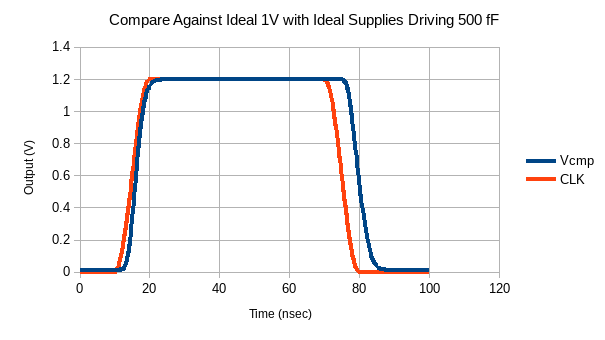
\includegraphics[width=\linewidth]{strongarm_data/strongarm-trans.png}
\end{figure}
\end{frame}

\begin{frame}{Transfer Characteristics}
\begin{figure}
    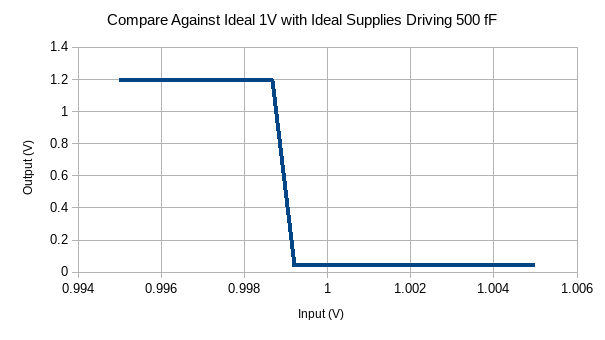
\includegraphics[width=\linewidth]{strongarm_data/strongarm-xfer.png}
\end{figure}
\end{frame}

\begin{frame}{Clocking with the PGA and ADC}
\begin{itemize}
\item Synchronized PGA "$\phi_1$", the "sample" phase, with the ADC's "compare" phase, and the PGA's "$\phi_2$, or "amplify", with the ADC's "load" phase
\item $\phi_1$ and $\phi_2$ are 5 $\mu$s each, with rise and fall times of 10 ns, and thus the clock period of 10 $\mu$s satisfies the 100ksamples/s required by spec
\item ADC clock (10MHz) is equal to digital clock
\item We deliberately delayed the digital clock by 10ns so that it would not interfere with rise/fall times of $\phi_1$ and $\phi_2$, as it was previously causing the ADC to raise the MSB 100\% of the time
\end{itemize}
\end{frame}
%

\section{Conclusions}
\subsection{Lessons Learned}
\begin{frame}{Lessons Learned}
\begin{itemize}
\item Make running tests easy, test often
\item There are no such things as 'small' changes
\item Having a good band gap is \textbf{extremely} important for the performance of the circuit
\begin{itemize}
\item PSR + start-up circuit
\end{itemize}
\item Small capacitors and leaky transistors are problematic for maintaining a voltage
\begin{itemize}
\item Charge pump
\end{itemize}
\item Erratic or spiky behavior can be handled with fast amps
\begin{itemize}
\item Use smaller lengths and bigger widths
\end{itemize}
\end{itemize}
\end{frame}

\end{document}
